\section{Introduction}
Today, learning systems have gain significant attention in the literature for the overwhelming popularity of machine-learning (ML) related workloads, be it in a private cluster, datacenter, or in the public cloud.

While most of work to date in the systems and architecture community has focused on improving the efficiency of evaluating trained models. This makes sense given that a model is trained only once but can be used many times for inference. However, arriving at a trained model frequently requires experimentation, and thus multiple training runs, each of which may take days. Accelerating the training process lets ML scientists iterate faster and design better model.

Traditionally, training has been viewed as a compute-bound problem, best done in a single large compute node with many accelerators. However, the ever-growing data volume pushes for monster-sized models to a scale where even the exponentiation of compute power growth in single device couldn't handle. As ML models get bigger, training time gets prohibitively longer. Timely training requires exploiting parallelism with a distributed system.

\begin{table}
\centering
\begin{tabular}{|c|c|c|c|c|}
  \hline
  Models & Complexity & Size & Time & Configuration \\
  \hline
  Linear Regression~\cite{seber2012linear} & O($D^3+ N^2D$) & Small & Short & CPU \\
  \hline
  SVM~\cite{wang2005support} & O($N^2D^2$) & Small & Short & CPU \\
  \hline
  GBDT~\cite{friedman2001greedy} & O($TLFN$) & Small & Short & A few CPUs \\
  \hline
  \hline 
  AlexNet~\cite{alexnet}   & 0.0058 & 48M & 6 days  & 2x GTX 580\\
  \hline
  ZFNet~\cite{ZFNet}   & 0.0062  &  $\approx$48M  & 12 days  & GTX 580\\
  \hline
  VGGNet~\cite{VGGNet}   & 0.12  & 137M & 15 days & 4x Titan Black\\
  \hline
  GoogleNet~\cite{GoogleNet}   & 0.03  & 9M & 7 days & A few GPUs\\
  \hline
  ResNet~\cite{RESNET}   & 0.117 &  58M & 21 days & 8x GPUs\\
  \hline
  Xception~\cite{Chollet_2017}  & 5.0  & 22M & 30 days & 60x K80\\
  \hline
  \hline
  BERT~\cite{bert}  & 3.8 & 340M & 4 days & 16x TPUs v2 \\
  \hline
  GPT-2~\cite{GPT2}  & 248 & 1.5B & 7+ days~\cite{gpt2Time} & 256x TPUs v3 \\
  \hline
  \hline
%  Device Placement~\cite{mirhoseini2017device} 2017 & - & 27 hours & 80 GPU nodes  \\
%  \hline
  NAS~\cite{zoph2016neural}  & 31 & 86M & 28 days & 800 K40 GPUs\\
  \hline
  AlphaGoZero~\cite{silver2016mastering}  & 1800 & - & 1 day & 5000x TPUs \\
  \hline
\end{tabular}
\caption{A few representative machine learning techniques and models that support increasingly complex tasks (trees, support vector machines, neural networks) and their complexities to train (pfs-day, or days to train computing at 1 PFlop/s. 1PF/s roughly corresponds to 64 Tesla V100 GPUs FP32, or 8 with mixed-precision FP16, running at peak throughput), and their reported training time and the machines they are trained on. We used the same method of estimating complexity as in the original OpenAI blog post~\cite{AIandCom3:online} for the additional models in the table. $D$: features. $N$: samples. $L$: leaves per tree. $T$: number of trees to build.}
\label{table:trend}
\end{table}

Table~\ref{table:trend} gives a summary of how the machines learning models/techniques are getting so much more demanding in terms of compute resources, such that the use of hundreds or even thousands of machines and accelerators for weeks is commonplace. 

The most common way of exploiting parallelism, ``data'' parallelism, consists of a computation-heavy forward and backward phase and a communication-heavy parameter exchange phase. Efficient distributed training involves optimizing both stages. Many past work demonstrate the solution of accelerating these processes by building specialized hardware clusters with fast interconnects ~\cite{DBLP:journals/corr/abs-1711-00489, You:2018:ITM:3225058.3225069, DBLP:journals/corr/abs-1711-04325,jia2018highly,DBLP:journals/corr/abs-1811-05233,sun2019optimizing, ImageNetIn1Hour, firecaffe, phubsocc}. While the results are encouraging, as we shall see, faster hardware is not panacea: the unstreamlined software stack and unbalanced compute to communication resource allocation prohibits utilizing the full capability of the hardware, and the compute units are more likely than not waiting on the network because the latter simply cannot keep up. We expect the problem not going away on its own, because of the observed trend at which the network capability is growing is significantly outpaced by that of the compute resources (Figure~\ref{fig:accthroughput}).  

\begin{figure}
	\centering
	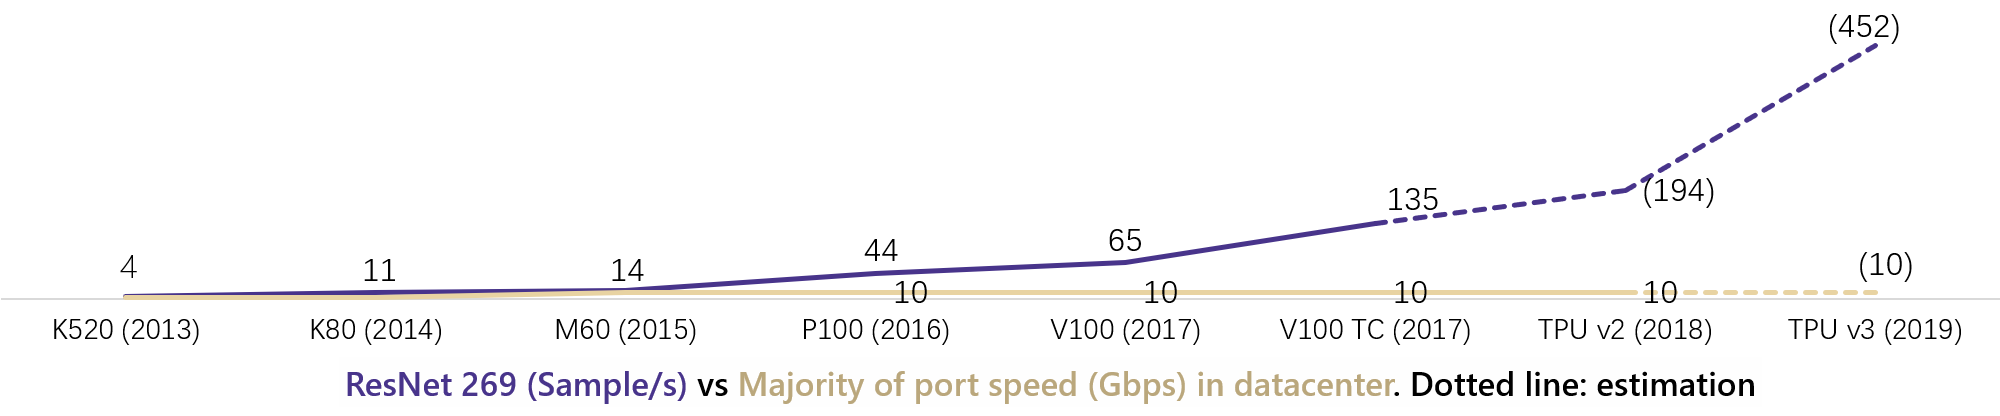
\includegraphics[width=\linewidth, trim=2 3 3 3,clip]{Figures/computevscomm.png}
	\caption{Throughput for an industry standard benchmark (ResNet) has seen an improvement of 35x, and is estimated to increase by 100x with latest accelerators. GPU performance tested with MxNet on EC2. TPU throughput estimated based on TensorCore's measured performance. Estimation for majority of the port speed of datacenters is based on~\cite{CISCOMarket}.}
	\label{fig:accthroughput}
\end{figure}

To tackle these problems, it is important to understand accelerating training in these specialized, privately-owned clusters does not complete the story: first, those hardware setups require steep investment and only a few have that luxury; second, it is much easier to thoroughly optimize the entire stack as we have control over the entire system. 

On the other hand, public cloud-based learning has become a popular, more accessible alternative, as all major cloud providers offer racks of nodes with specialized accelerators (such as GPUs, TPUs, and custom FPGAs)~\cite{GoogleCl74:online,MachineL50:online,DeepLear23:online,sagemaker,brainwave,Jouppi:2017:IPA:3079856.3080246,222611} for ML workloads. But at the same time, scalable training in the public cloud faces additional challenges - more than just an inefficient hardware/software stack. Even with modern frameworks and recent optimizations 
(e.g., gradient compression and quantization~\cite{lin2017deep, cntk1bt, lim20183lc}, latency-hiding~\cite{poseidon, jayarajan2019priority,hashemi2018tictac}, optimized communication libraries~\cite{facebook35:online, Operatio73:online, dmlcpsli50:online} and large batch optimizations~\cite{ImageNetIn1Hour}), distributed training at scale on the public cloud still incurs high overhead: up to 90\% of total training time can be wasted waiting on the network (Figure~\ref{fig:cloudOverhead}). While existing solutions focus solely on addressing the \textit{bandwidth} bottleneck, the cloud environments pose additional challenges (\textsection\ref{sec:challenges}). The hierarchical network structure breaks the usual assumption of link speed being uniform; multi-tenancy and the dynamic nature of the cloud traffic cause high variation in performance. All these add to the complexity of scaling up distributed training and can render existing solutions less effective~(\textsection\ref{sec:differentReductionAlgorithms}). These issues, coupled with the fact that the speed at which the throughput of emerging accelerators is improving significantly outpaces that of the networking devices~\cite{luo2017motivating}, keep cloud-based training communication bound.